\documentclass[a4paper,12pt]{article}
\usepackage{amsmath, amssymb, graphicx, physics, hyperref, bm,amsthm}
\usepackage{geometry}
\geometry{a4paper, margin=1in}
\usepackage{titlesec}
\usepackage{tocloft}
\usepackage{wrapfig}

\newtheorem{theorem}{Theorem}
\newtheorem{lemma}{Lemma}

\begin{document}

\title{Mathematical Foundations of Optical Interferometry: Embedding Arbitrary Matrices into Mach-Zehnder Interferometers}
\author{Marc DeCarlo, Santiago Sosa}
\date{\today}
\maketitle

\tableofcontents

\section{Introduction}

This section provides a rigorous mathematical derivation of beam splitters, mirrors, Mach-Zehnder interferometers (MZIs), and their use in performing matrix multiplications. We also present the complex Schur decomposition and its role in embedding an arbitrary matrix into an MZI-based optical computing architecture.

\section{Mathematical Description of Optical Components}

\subsection{Beam Splitters}
A 50:50 beam splitter transforms the input field amplitudes as follows:
\begin{equation}
B = \frac{1}{\sqrt{2}} \begin{bmatrix} 1 & i \\ i & 1 \end{bmatrix}.
\end{equation}
This matrix ensures energy conservation and unitary behavior.

\subsubsection{Proof of Beam Splitter Matrix}
To show that the beam splitter matrix is unitary, we compute:
\begin{equation}
B^H B = \frac{1}{2} \begin{bmatrix} 1 & -i \\ -i & 1 \end{bmatrix} \begin{bmatrix} 1 & i \\ i & 1 \end{bmatrix} = I.
\end{equation}
This confirms that the beam splitter transformation preserves norm and is unitary.
\subsection{\textbf{Derivation of the Beam Splitter Matrix}}
A \textbf{50:50 beam splitter} takes an incident optical field and \textbf{splits it into two paths} while introducing a phase shift in the reflected component. 

\subsubsection{\textbf{Define the Input and Output Fields}}
Let the input complex field amplitudes for the two ports be:
\begin{equation}
    \begin{bmatrix} E_1^{\text{in}} \\ E_2^{\text{in}} \end{bmatrix}
\end{equation}
where:
- \( E_1^{\text{in}} \) represents the field entering from port 1.
- \( E_2^{\text{in}} \) represents the field entering from port 2.

The output fields \( E_1^{\text{out}}, E_2^{\text{out}} \) are related to the input by a transformation matrix \( B \):

\begin{equation}
    \begin{bmatrix} E_1^{\text{out}} \\ E_2^{\text{out}} \end{bmatrix} = B \begin{bmatrix} E_1^{\text{in}} \\ E_2^{\text{in}} \end{bmatrix}
\end{equation}

\subsubsection{\textbf{Form of the Beam Splitter Matrix}}
By experimental observation and symmetry considerations, the transformation must be \textbf{unitary} and \textbf{preserve energy}. We assume the general form:

\begin{equation}
B =
\begin{bmatrix}
    t & r \\
    r & t
\end{bmatrix}
\end{equation}

where:
- \( t \) is the \textbf{transmission coefficient}.
- \( r \) is the \textbf{reflection coefficient}.

\subsubsection{\textbf{Enforcing Energy Conservation}}
Energy conservation in an optical system requires that the total intensity (power) remains unchanged:

\begin{equation}
    |E_1^{\text{out}}|^2 + |E_2^{\text{out}}|^2 = |E_1^{\text{in}}|^2 + |E_2^{\text{in}}|^2.
\end{equation}

This implies that \( B \) must be \textbf{unitary}, meaning:

\begin{equation}
    B^\dagger B = I.
\end{equation}

Expanding,

\begin{equation}
\begin{bmatrix}
    t^* & r^* \\
    r^* & t^*
\end{bmatrix}
\begin{bmatrix}
    t & r \\
    r & t
\end{bmatrix}
=
\begin{bmatrix}
    |t|^2 + |r|^2 & t^* r + r^* t \\
    r^* t + t^* r & |t|^2 + |r|^2
\end{bmatrix}
=
\begin{bmatrix}
    1 & 0 \\
    0 & 1
\end{bmatrix}.
\end{equation}

From this, we obtain two conditions:

\textbf{1. Energy Conservation Condition:}
   \begin{equation}
   |t|^2 + |r|^2 = 1.
   \end{equation}

\textbf{2. Cross-Term Cancellation:}
   \begin{equation}
   t^* r + r^* t = 0.
   \end{equation}

Since \( t \) and \( r \) are complex numbers, we let:

\begin{equation}
    t = \frac{1}{\sqrt{2}}, \quad r = \frac{i}{\sqrt{2}}.
\end{equation}

which satisfies the unitary condition:

\begin{equation}
\left( \frac{1}{\sqrt{2}} \right)^2 + \left( \frac{i}{\sqrt{2}} \right)^2 = \frac{1}{2} + \frac{1}{2} = 1.
\end{equation}

Thus, the \textbf{beam splitter matrix} is:

\begin{equation}
B =
\frac{1}{\sqrt{2}}
\begin{bmatrix}
    1 & i \\
    i & 1
\end{bmatrix}.
\end{equation}

\subsubsection{\textbf{Verification of Unitarity}}
To verify that this matrix is \textbf{unitary}, we compute:

\begin{equation}
    B^\dagger B =
    \frac{1}{\sqrt{2}}
    \begin{bmatrix}
        1 & -i \\
        -i & 1
    \end{bmatrix}
    \frac{1}{\sqrt{2}}
    \begin{bmatrix}
        1 & i \\
        i & 1
    \end{bmatrix}.
\end{equation}

Expanding:

\begin{equation}
\frac{1}{2}
\begin{bmatrix}
    1 + 1 & 0 \\
    0 & 1 + 1
\end{bmatrix}
=
\begin{bmatrix}
    1 & 0 \\
    0 & 1
\end{bmatrix}.
\end{equation}

Thus, the matrix is \textbf{unitary}, completing the proof.


\subsection{Mirrors}
Mirrors introduce a phase shift upon reflection:
\begin{equation}
M = \begin{bmatrix} e^{i\phi} & 0 \\ 0 & e^{i\psi} \end{bmatrix},
\end{equation}
where \( \phi \) and \( \psi \) are phase shifts depending on the optical path.

\section{Mach-Zehnder Interferometer (MZI)}
\begin{figure}[h]
    \centering
    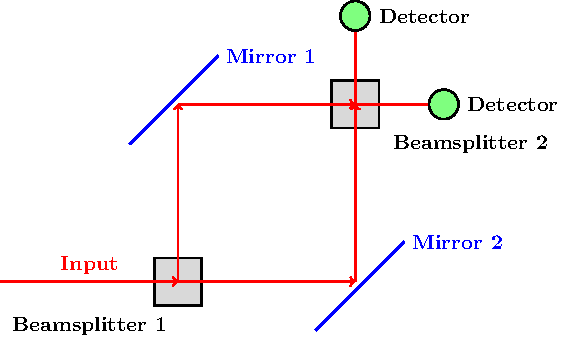
\includegraphics[width=0.8\textwidth]{mzi_diagram.pdf}
    \caption{Mach-Zehnder Interferometer Diagram}
    \label{fig:mzi}
\end{figure}
An MZI consists of two beam splitters and phase shifters, modeled as:
\begin{equation}
U_{\text{MZI}} = B P B,
\end{equation}
where \( P \) is a diagonal phase shift matrix:
\begin{equation}
P = \begin{bmatrix} e^{i\theta_1} & 0 \\ 0 & e^{i\theta_2} \end{bmatrix}.
\end{equation}
The resulting transformation matrix remains unitary.

\section{Complex Schur Decomposition}
For any arbitrary matrix \( A \in \mathbb{C}^{n \times n} \), there exists a unitary decomposition:
\begin{equation}
A = Q T Q^H,
\end{equation}
where:
\begin{itemize}
    \item \( Q \) is a unitary matrix (can be implemented with fixed beam splitters),
    \item \( T \) is an upper triangular matrix (implemented using phase shifters).
\end{itemize}
The \textbf{Schur Decomposition} states that for any square complex matrix \( A \in \mathbb{C}^{n \times n} \), there exists a unitary matrix \( Q \) and an upper triangular matrix \( T \) such that:
\begin{equation}
    A = Q T Q^H,
\end{equation}
where:
\begin{itemize}
    \item \( Q \) is a \textbf{unitary matrix} (\( Q^H Q = I \)).
    \item \( T \) is an \textbf{upper triangular matrix} whose diagonal entries are the eigenvalues of \( A \).
    \item \( Q^H \) is the Hermitian transpose of \( Q \).
\end{itemize}

This decomposition is fundamental in numerical linear algebra, particularly for computing eigenvalues, solving matrix equations, and designing optical matrix multiplications.

\subsection{\textbf{Preliminary Lemmas}}

Before proving the Schur decomposition, we state two important lemmas.

\begin{lemma}[Unitary Similarity Preserves Eigenvalues]
    If \( B = U A U^H \) for some unitary matrix \( U \), then \( A \) and \( B \) have the same eigenvalues.
\end{lemma}

\begin{proof}
    Suppose \( \lambda \) is an eigenvalue of \( A \) with eigenvector \( v \), so:
    \[
    A v = \lambda v.
    \]
    Multiplying both sides by \( U \),
    \[
    U A v = \lambda U v.
    \]
    Setting \( w = U v \), we get:
    \[
    B w = (U A U^H) U v = U A v = \lambda w.
    \]
    Thus, \( B \) has the same eigenvalues as \( A \).
\end{proof}

\begin{lemma}[Existence of a Unitary Basis for an Eigenvector]
    Every complex matrix \( A \in \mathbb{C}^{n \times n} \) has at least one eigenvector that can be extended to form a unitary basis of \( \mathbb{C}^n \).
\end{lemma}

\begin{proof}
    By the \textbf{fundamental theorem of algebra}, every square complex matrix has at least one eigenvalue \( \lambda_1 \) with a corresponding eigenvector \( v_1 \). The Gram-Schmidt process can be applied to extend \( v_1 \) into an orthonormal basis \( \{ v_1, v_2, \dots, v_n \} \), which forms a unitary matrix.
\end{proof}

\subsection{\textbf{Proof of the Schur Decomposition Theorem}}

\begin{theorem}[Schur Decomposition]
    For any complex matrix \( A \in \mathbb{C}^{n \times n} \), there exists a unitary matrix \( Q \) and an upper triangular matrix \( T \) such that:
    \[
    A = Q T Q^H.
    \]
\end{theorem}

\begin{proof}
    We prove this by induction on the size \( n \) of the matrix \( A \).

    \textbf{Base Case (n = 1):} A \( 1 \times 1 \) matrix is trivially its own Schur form.

    \textbf{Inductive Step:} Assume that for any \( (n-1) \times (n-1) \) complex matrix, there exists a unitary matrix \( Q_{n-1} \) such that:
    \[
    Q_{n-1}^H A_{n-1} Q_{n-1} = T_{n-1},
    \]
    where \( T_{n-1} \) is upper triangular.

    Now, consider an \( n \times n \) matrix \( A \). By the eigenvalue existence theorem, let \( v_1 \) be an eigenvector of \( A \) corresponding to eigenvalue \( \lambda_1 \). Extend \( v_1 \) to form a unitary basis \( Q_1 = [v_1, v_2, \dots, v_n] \).

    Construct the unitary matrix:
    \[
    Q = [v_1, Q_{n-1}],
    \]
    where \( Q_{n-1} \) orthonormally spans the remaining space.

    Applying unitary similarity,
    \[
    Q^H A Q =
    \begin{bmatrix}
        \lambda_1 & w^H \\
        0 & A'
    \end{bmatrix},
    \]
    where \( w \) is some row vector and \( A' \) is an \( (n-1) \times (n-1) \) matrix.

    By the induction hypothesis, \( A' \) has a Schur decomposition:
    \[
    A' = Q_{n-1} T' Q_{n-1}^H.
    \]

    Substituting back, we get:
    \[
    Q^H A Q =
    \begin{bmatrix}
        \lambda_1 & w^H \\
        0 & Q_{n-1} T' Q_{n-1}^H
    \end{bmatrix}.
    \]

    Since \( Q_{n-1} \) is unitary, it preserves triangularity:
    \[
    T =
    \begin{bmatrix}
        \lambda_1 & w^H \\
        0 & T'
    \end{bmatrix},
    \]
    which is upper triangular. Thus, we obtain:
    \[
    A = Q T Q^H.
    \]
\end{proof}



\section{Embedding an Arbitrary Matrix into an MZI for Matrix Multiplication}
Given an arbitrary \( 2 \times 2 \) matrix \( A \), we compute the Schur decomposition:
\begin{equation}
A = Q T Q^H.
\end{equation}

\subsection{Implementing Q Using Fixed Beam Splitters}
Since MZIs implement unitary matrices of the form:
\begin{equation}
B = \frac{1}{\sqrt{2}} \begin{bmatrix} 1 & i \\ i & 1 \end{bmatrix},
\end{equation}
we can directly use an MZI network to implement \( Q \) and \( Q^H \).

\subsection{Implementing T Using Phase Shifters}
Since \( T \) is upper triangular with eigenvalues on the diagonal:
\begin{equation}
T = \begin{bmatrix} e^{i\theta_1} & t_{12} \\ 0 & e^{i\theta_2} \end{bmatrix},
\end{equation}
this can be implemented by setting appropriate phase shifts within the MZI.

\subsection{Final Optical Implementation}
\begin{enumerate}
    \item Apply \( Q^H \) using a fixed MZI beam splitter network.
    \item Apply \( T \) using phase shifters.
    \item Apply \( Q \) using a second MZI beam splitter network.
\end{enumerate}

Thus, \( A x \) is implemented optically as:
\begin{equation}
A x = Q T Q^H x.
\end{equation}

\end{document}
